\chapter{Introduction}

The digital CMS pixel chip, colloquially called \glsreset{ROC}\gls{ROC}, consists of 52$\times$80~pixels. Electrically they are organized in 26 double columns, each having 2$\times$80~pixels. One double column is controlled by a periphery which has buffers for time-stamps and data. There are 24~time-stamp buffers (8~bit wide) and 80~data buffers, see Fig.~\ref{fig:ROCimage}

\begin{figure}[hbtp]
	\begin{center}
	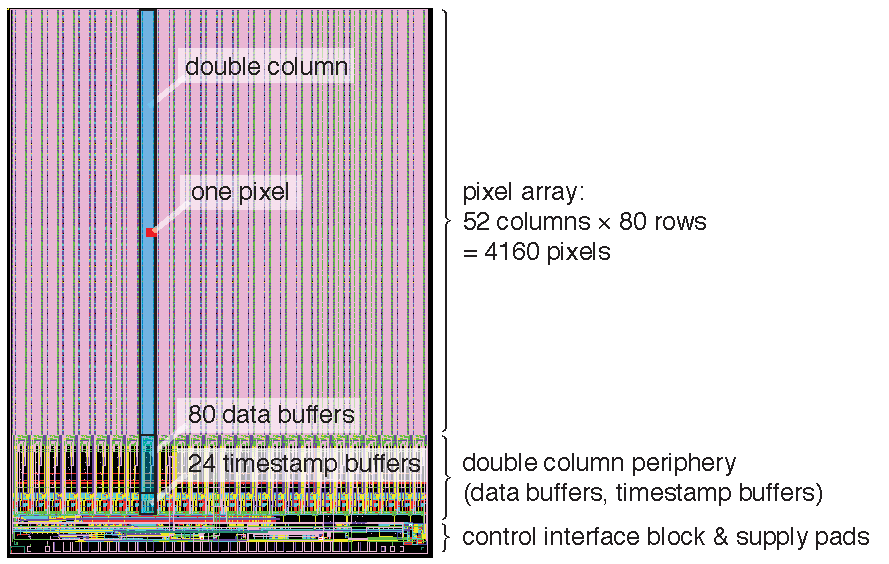
\includegraphics[width=.9\textwidth]{img/ROCimage.pdf}
	\end{center}
	\caption{Pixel chip arrangement. The image shows the full layout of a pixel chip. Highlighted are the areas of a single pixel, double column, the data buffers and the timestamp buffers. The periphery and the supply pads are in charge to handle trigger information, buffer data of recent pixel data and handle the communication with the outer world.}
	\label{fig:ROCimage}
\end{figure}

%==============================================================================
\chapter{Pad layout}

Fig.~\ref{fig:ROCpadschematic} shows the main wire-bond pads and their names. Table~\ref{tab:ROCpinout} describes the meaning of the signals. 

\begin{figure}[hbtp]
	\begin{center}
	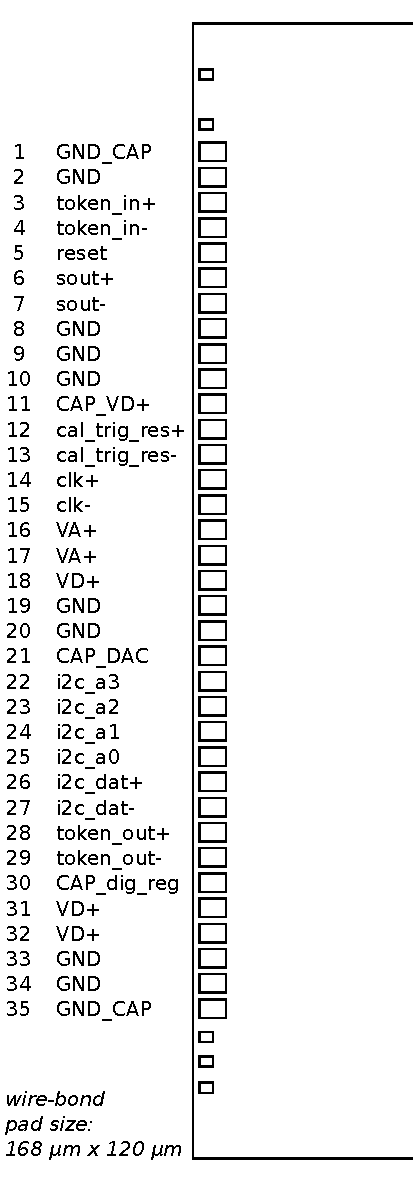
\includegraphics[width=.3\textwidth]{img/ROC_padschema.pdf}
	\end{center}
	\caption{Location and names of wire-bond pads on the chip.}
	\label{fig:ROCpadschematic}
\end{figure}

\begin{table}[h]
    \begin{center}
	\caption{\textbf{List of wire-bond pads.} }
	\label{tab:ROCpinout}

	\bigskip

	{\scriptsize
	\begin{tabular}{clcl}
	\toprule %-------------------------------------------------------------------------------------------------
	Pin\# & Name         & Type & Description \\
	\midrule %-------------------------------------------------------------------------------------------------
	 1 & GND\_CAP        & out & External filter capacitances, connected to GND internally in the chip \\
	\midrule %-------------------------------------------------------------------------------------------------
	 2 & GND             & in  & Ground \\
	\midrule %-------------------------------------------------------------------------------------------------
	 3 & token\_in+      & in  & \multirow{2}{*}{Readout token} \\
	 4 & token\_in-      & in  & \\
	\midrule %-------------------------------------------------------------------------------------------------
	 5 & reset           & in  & Hard chip reset, resets all double columns, \isqc{}, DAC's \\
	\midrule %-------------------------------------------------------------------------------------------------
	 6 & sout+           & out & \multirow{2}{*}{Serial output of data} \\
	 7 & sout-           & out & \\
	\midrule %-------------------------------------------------------------------------------------------------
	 8 & GND             & in  & \multirow{3}{*}{Ground}  \\
	 9 & GND             & in  & \\
	10 & GND             & in  & \\
	\midrule %-------------------------------------------------------------------------------------------------
	11 & CAP\_VD+        & out & External capacity filtering unregulated VD, internally connected to pad 18 \\
	\midrule %-------------------------------------------------------------------------------------------------
	12 & cal\_trig\_res+ & in  & \multirow{2}{*}{Combined signal: calibrate/trigger/reset} \\
	13 & cal\_trig\_res- & in  & \\
	\midrule %-------------------------------------------------------------------------------------------------
	14 & clk+            & in  & \multirow{2}{*}{40\,MHz clock} \\
	15 & clk-            & in  & \\
	\midrule %-------------------------------------------------------------------------------------------------
	16 & VA+             & in  &\multirow{2}{*}{Analog voltage +1.5\,V} \\
	17 & VA-             & in  & \\
	\midrule %-------------------------------------------------------------------------------------------------
	18 & VC+             & in  & Input to supply the comparators with +2.5\,V (same as VD+), see also pad 11 \\
	\midrule %-------------------------------------------------------------------------------------------------
	19 & GND             & in  & \multirow{2}{*}{Ground} \\
	20 & GND             & in  & \\
	\midrule %-------------------------------------------------------------------------------------------------
	21 & CAP\_DAC        & out & External capacity filtering the internally regulated voltage supplying th DAC's \\
	\midrule %-------------------------------------------------------------------------------------------------
	22 & i2c\_a3         & in  & \multirow{4}{*}{Chip address bits 0 to 3} \\
	23 & i2c\_a2         & in  & \\
	24 & i2c\_a1         & in  & \\
	25 & i2c\_a0         & in  & \\
	\midrule %-------------------------------------------------------------------------------------------------
	26 & i2c\_dat+       & in  & \multirow{2}{*}{\isqc{} data SDA} \\
	27 & i2c\_dat-       & in  & \\
	\midrule %-------------------------------------------------------------------------------------------------
	28 & token\_out+     & out & \multirow{2}{*}{Readout token output} \\
	29 & token\_out-     & out & \\
	\midrule %-------------------------------------------------------------------------------------------------
	30 & CAP\_dig\_reg   & out & External capacitance filtering VD regulated \\
	\midrule %-------------------------------------------------------------------------------------------------
	31 & VD+             & in  & \multirow{2}{*}{Digital voltage +2.5\,V} \\
	32 & VD-             & in  & \\
	\midrule %-------------------------------------------------------------------------------------------------
	33 & GND             & in  & \multirow{2}{*}{Ground}\\
	34 & GND             & in  & \\
	\midrule %-------------------------------------------------------------------------------------------------
	35 & GND\_CAP        & out & External filter capacitances, connected to GND internally in the chip \\
	\bottomrule %-------------------------------------------------------------------------------------------------
	\end{tabular}
	}
    \end{center}
\end{table}

%==============================================================================
\chapter{DAC's and registers}

The chip has 12 DAC's and 2 registers plus trim bits for each pixel. Table~\ref{tab:DecBinHex} lists the DAC's and registers used in the analog signal chain. Fig.~\ref{fig:ROCDACschematic} illustrates the meaning of the DAC's along the signal chain.

\begin{table}[h]
    \begin{center}
	\caption{\textbf{DAC and registers.} The values being sent to the ROC are 4 or 8 bit words.}
	\label{tab:DecBinHex}

	\bigskip

	{\scriptsize
	\begin{tabular}{lrccrrrl}
	\toprule
	Name & addr & unit & \# bits & \multicolumn{1}{p{0.8cm}}{Min Value} & \multicolumn{1}{p{0.8cm}}{Max Value} & \multicolumn{1}{p{1.2cm}}{Recomm. DAC Value} & Description \\ 
	\midrule
	\multicolumn{ 8}{l}{\textbf{Voltage Regulators}} \\ 
	Vdd         &  1 &   mV    & 4 & 1700 & 2100 & 6 & Voltage regulator for digital supply \\ 
	Iana        &  2 &   mA    & 8 & 5 & 65 & 90 & Current regulator for analog supply \\ 
	Vsh         &  3 &   mA    & 8 & 1 & 14 & 40 & Current regulator for sample \& hold circuit \\ 
	Vcomp       &  4 &   mV    & 4 & 1800 & 2100 & 12 & Voltage regulator for comparator \\ 
	\midrule
	\multicolumn{ 8}{l}{\textbf{Analog control in pixel unit cell}} \\ 
	FBPre       &  7 &   mV    & 8 & 400 & 1300 & 60 & Preamplifier feedback  \\ 
	FBSh        &  9 &   mV    & 8 & 400 & 1300 & 60 & Shaper feedback \\ 
	HoldDel     & 10 &   mV    & 8 & -1500 & -500 & 117 & Hold delay \\ 
	TrimScale   & 11 &   mV    & 8 & -710 & -400 & 29 & Pixel trimming \\ 
	GlobalThr   & 12 &   mV    & 8 & -1500 & -600 & 60 & Comparator threshold \\ 
	%\midrule
	%\multicolumn{ 8}{l}{\textbf{Pixel Readout}} \\ 
	%VIbias\_bus & 13 & $\mu$A  & 8 & 0 & 12 & 5 & Digital bus receiver \\ 
	%VIbias\_sf  & 14 & $\mu$A  & 4 & 0 & 50 & 6 & Analog bus receiver \\ 
	%VIColOr     & 22 & $\mu$A  & 8 & 0 & 200 & 20 & Current limiter \\ 
	\midrule
	\multicolumn{ 8}{l}{\textbf{Double Column Readout}} \\ 
	%VOffsetOp   & 15 &   mV    & 8 & 1000 & 1500 & 90 & Charge amplifier offset \\ 
	PHOffset    & 17 &   mV    & 8 & 1000 & 1500 & 76 & Voltage amplifier offset \\ 
	%VIon        & 18 & $\mu$A  & 8 & 0 & 100 & 115 & Voltage amplifier bias current \\ 
	\midrule
	\multicolumn{ 8}{l}{\textbf{Chip Readout}} \\ 
	ADCpower    & 19 & mV & 8  & 600 & 1050 & 100 & ADC comparator voltage \\ 
	PHscale     & 20 & $\mu$A  & 8 & 0 & 12 & 160 & ADC reference current \\ 
	\midrule
	\multicolumn{ 8}{l}{\textbf{Others}} \\ 
	Vcal        & 25 & mV      & 8 & 0 & 260/1800 & 150 & Calibrate pulse height, see also section~\ref{sec.5.3.5} \\ 
	CalDel      & 26 & nsec    & 8 & 55 & 205 &  & See chapter~\ref{sec.7} \\ 
	WBC         & 254 & clocks & 8 & 0 & 255 &                 >70 & Trigger latency \\ 
	CCR         & 253 &        & 8 &  &  &  & See section~\ref{sec.5.3.5} \\ 
	\bottomrule
	\end{tabular}
	}
    \end{center}
\end{table}

\begin{figure}[hbtp]
	\begin{center}
	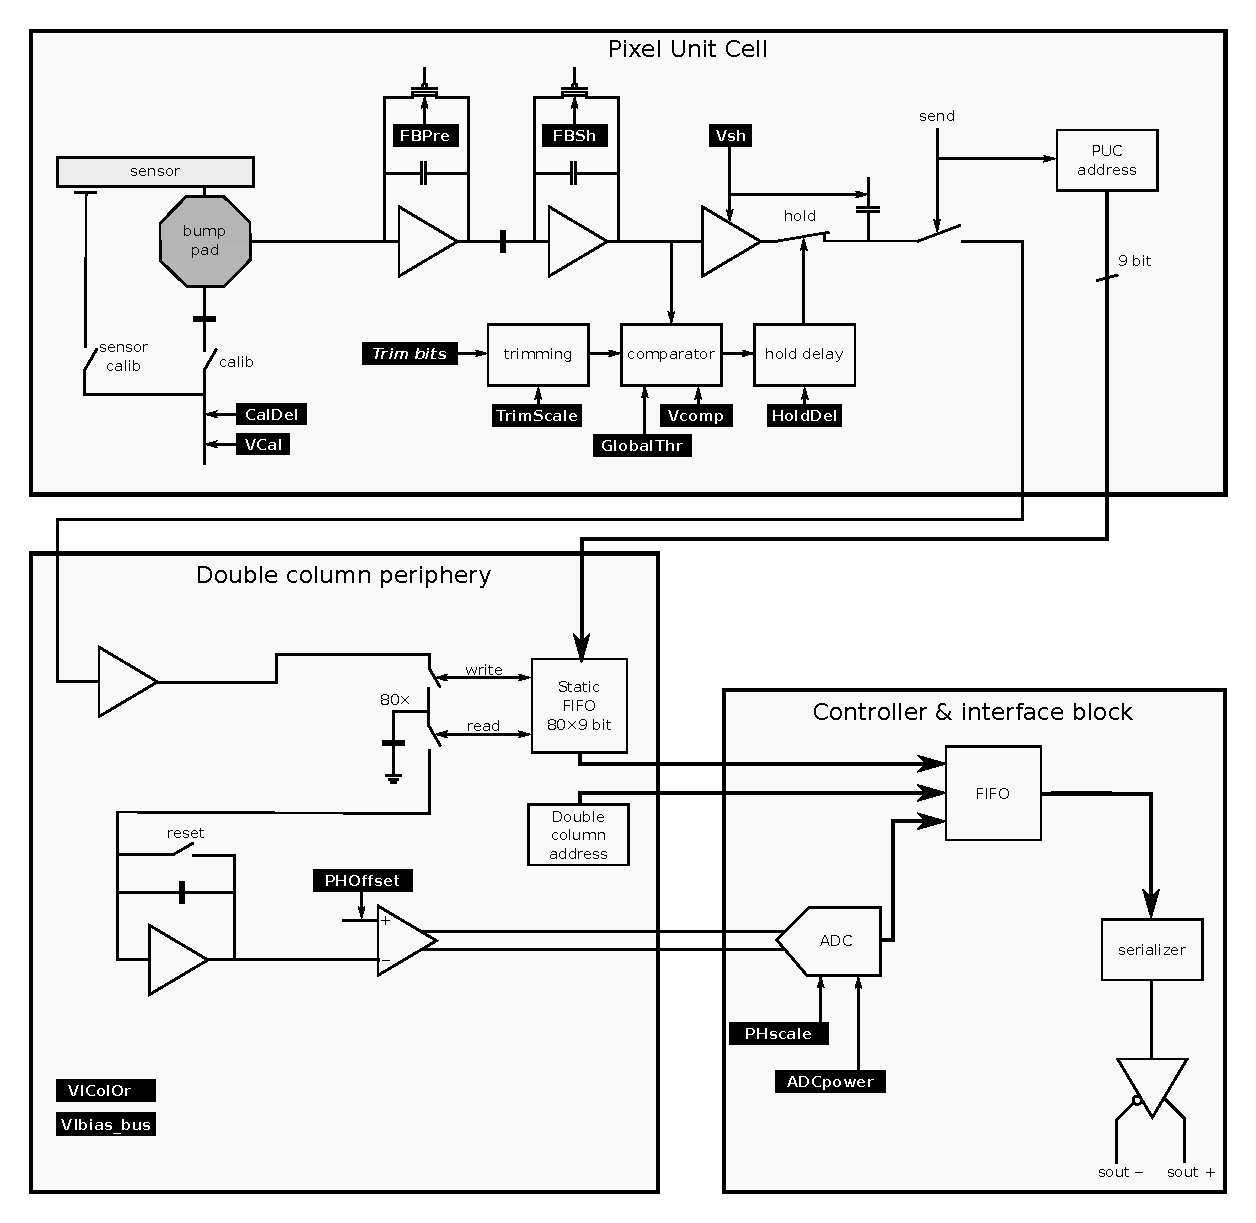
\includegraphics[width=.9\textwidth]{img/ROC_DACschema.pdf}
	\end{center}
	\caption{Pixel chip schemtaic with DAC's. }
	\label{fig:ROCDACschematic}
\end{figure}


